\chapter{陆地生态系统碳循环模型开放式对比框架}
\label{cha:3}

根据第\ref{chap:model}章的分析,陆地生态系统碳循环模型具有种类多样、参数复杂、难以应用的特点,模拟过程参与的要素众多(如GPP、NPP、NEP、Biomass、LAI等),模拟站点丰富,数据需求量大、难以搜集。这些因素都共同阻碍了碳循环模型的应用和发展,开展模型对比工作往往十分艰巨,像CMIP项目那样,各个模式开发组共同参与进来才能更顺利地完成。但是传统的对比框架也面临着一些问题,它将模型计算和对比过程都放在本地计算机运行,模型难以共享和重用,对比过程不够公开,换一套数据或研究区域就难以重现或重复,这些都是由于基于本地计算的对比框架所导致的。针对这一问题,本章旨在设计一个开放式的对比框架,支持将各种对比资源以微服务的形式开放地接入进来,实现可共享、可重用、公开化的陆地生态系统碳循环模型的对比。

本章首先分析了陆地生态系统碳循环模型的对比情景,并从中归纳总结出“对比话题——对比方案——对比任务”的三部流程;其次详细探讨了对比过程中的需要接入的地理资源组件库,包括有模型服务资源库、数据服务资源库、单位量纲资源库、数据处理服务资源库、对比服务资源库,并设计了对应接口来满足相应资源的接入,实现了对比资源的标准一致性和可扩展性;然后设计了分布式的网络系统架构,将整体复杂的系统功能分割为三部分,实现了功能的解耦和系统的稳定和;最后通过科学工作流引擎支持网络环境下对比流程地自动化执行。
本系统的整体架构如图\ref{fig:CMIP-architecture}所示。

\begin{figure}[!htbp]
    \centering
    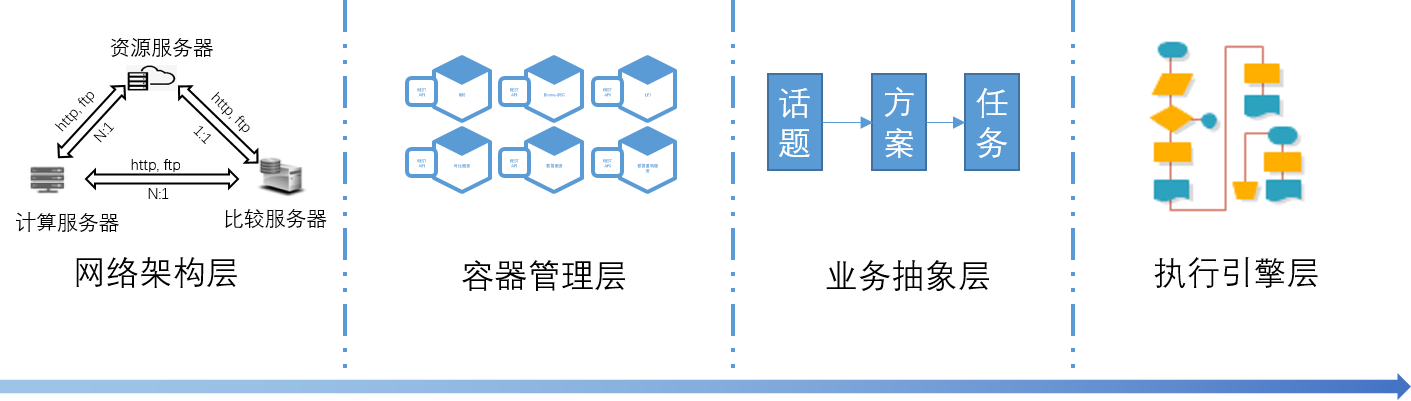
\includegraphics[width=.85\textwidth]{CMIP-architecture}
    \caption{陆地生态系统碳循环模型开放式对比框架}
    \label{fig:CMIP-architecture}
\end{figure}

\section{陆地生态系统碳循环模型对比情景和业务分析归纳}
\subsection{对比情景分析和总结}
\label{sec:scene}
% TODO 根据实验前提,详细介绍对比方案中的情景
陆地生态系统碳循环模型的应用广泛,未来的发展方向也主要停留在以下几个关键问题上:
\begin{enumerate}[(1)]
\item \textbf{陆地生态系统碳循环模型对历史植被生长的模拟}

在CMIP5和CMIP6的设计中,都设定了历史情景模拟,即根据历史时期的太阳常数、温室气体浓度、臭氧浓度、气溶胶浓度等观测资料来模拟气候因子,是气候系统模式参与CMIP项目的必要实验。而陆地生态系统碳循环模型作为气候系统模式机理中的一个子过程,也需要对历史时期进行模拟,来评估模型的模拟能力。历史情景分析是最常见的模拟情景,本文将在实验案例中详细介绍模拟结果。

\item \textbf{陆地生态系统碳循环模型的未来预测情景}
% 参考顾雪峰博士论文

在CMIP5和CMIP6中也设定了未来气候情景分析,即预测未来CO2浓度和气候因子(温度、降水)等指标的变化情况。在陆地生态系统碳循环模型对植被生产力的模拟方面,未来情景设定为气温、降水、CO2浓度的变化对植被生产力的影响,即研究陆地生态系统碳循环模型对气候变化(如温度、降水等)和CO2浓度的响应。CMIP5对未来100年全球气候变化的研究结果表明,全球平均气温从1990年到2100年上升$1.4\sim5.8^{\circ}C$~\cite{王绍武1995未来}~\cite{秦大河2003气候变化的事实与影响及对策};全球平均降水将会增加,但是降水格局也发生了很大的变化,即有些地区降水增加,有些地区降水减少;未来大气CO2浓度最大升高到当前的2倍~\cite{griggs2002climate}。根据这些预测的未来气候情景,对温度、降水和CO2浓度的变化做出变量组合,表~\ref{tab:future-scene}可以表示一种参考的组合。

% \hspace*{2cm}
\begin{table}[!htbp]
    \centering
    \caption{陆地生态系统碳循环模型的未来预测情景参数设定}
    \label{tab:future-scene}
    \begin{threeparttable}
        \begin{tabular}{lll}
            \Xhline{2pt}
            {\textbf{因素}} & {\textbf{值}} & {\textbf{标记}} \\
            \Xhline{2pt}
            \multirow{4}{*}{\textbf{气温}} & 不变 & $Temp_{0}$ \\
            & +2$^{\circ}C$ & $Temp_{1}$ \\
            & +4$^{\circ}C$ & $Temp_{2}$ \\
            & +6$^{\circ}C$ & $Temp_{3}$ \\
            \hline
            \multirow{7}{*}{\textbf{降水}} & 不变 & $Prec_0$ \\
            & 全年+10\% & $Prec_{+10}$ \\
            & 全年-10\% & $Prec_{-10}$ \\
            & 全年+20\% & $Prec_{+20}$ \\
            & 全年-20\% & $Prec_{-20}$ \\
            & 全年+30\% & $Prec_{+30}$ \\
            & 全年-30\% & $Prec_{-30}$ \\
            \hline
            \multirow{2}{*}{\textbf{CO2浓度}} & 不变 & $CO2_0$ \\
            & 两倍 & $CO2_{*2}$ \\
            \hline
            \multirow{4}{*}{\textbf{多因素}} & 温度增加、降水增加 & $Temp_{3} + Prec_{+10}$ \\
            & 温度增加、降水减少 & $Temp_{3} + Prec_{-10}$ \\
            & 温度增加、降水增加、CO2浓度翻倍 & $Temp_{3} + Prec_{+10} + CO2_{*2}$ \\
            & 温度增加、降水减少、CO2浓度翻倍 & $Temp_{3} + Prec_{-10} + CO2_{*2}$\\
            \Xhline{2pt}
        \end{tabular}
    \end{threeparttable}
\end{table}

\item \textbf{陆地生态系统碳循环模型的敏感性分析情景}
% 和对温度、降水、CO2的响应比较像,这里针对的是模型参数

在模型评价中,不确定分析研究的是模型参数、驱动变量等不确定性因素发生变化时,所引起的模型模拟结果的变化和变化程度。敏感性分析是模型不确定分析的一种常用方法,它用来研究和预测不确定性因素发生变化时,对模型结果影响程度的分析方法,又称为灵敏度分析。敏感性分析通常用来评估模型参数的重要性,分为总体敏感性分析和局部敏感性分析。局部敏感性分析相对来说更加简单,他分析单个模型参数对模拟结果的影响,但是他忽略了模型之间多个参数的相互作用对模拟结果的影响;全局敏感性分析不仅分析单个参数对模拟结果的影响,还分析参数之间的相互作用对结果的总影响,但计算起来比较复杂,耗费时间。
在本文中,将敏感性分析也理解为一种对比情景,即在不同的模型参数下模拟结果的对比,可以与正常模拟与观测数据的对比采用相同的对比方法。敏感性分析的情景设定需要从每个模型中选出一系列关键参数,根据参数的取值设定具体的情景,由于本文的研究重点不在于此,不做详细设定。

\item \textbf{陆地生态系统碳循环模型的参数校准情景}

碳循环模型的模拟精确度很大成分上依赖于模型参数的设定,目前在参数校准方面有人工校准和自动校准两种。人工校准通常有三种方法:对比实验、实验观测和文献查找;自动校准通过神经网络等各种模型进行校准。模型参数的校准可以理解为在不同模型参数下模型模拟结果的对比,因此可以作为对比的一种情景。

\end{enumerate}

\subsection{对比业务抽象和归纳}
% 对比分析、名词解释
% topic solution task
% 案例
% 意义:可共享 可重用

在进行对比业务抽象和归纳之前,先对本文中的一些名字做出解释:本文将GPP、NPP、NEP、Biomass、LAI等模拟指标称之为\textbf{对比要素};将模型对比过程中所需要的所有数据称之为\textbf{对比数据集},一套对比数据集包括有输入数据集、观测数据集。其中输入数据集由气象数据集、土壤数据集、植被功能类型数据集、DEM数据集等组成,每个具体的数据集可以选择可替换的模块,如气象数据集既可以采用MERRA 2再分析资料,又可以使用CRU再分析资料。在第\ref{sec:model-data}节中具体介绍的数据本文称之为标准对比数据集,作为系统分析的基础原始数据,而在其之上参照表~\ref{tab:future-scene}对数据进行的一系列修改,比如对温度$\pm2^{\circ}C$,对降水$\pm10\%$等,本文称之为衍生对比数据集。每一个模拟情景都有一套相对应的对比数据集。本文将参与对比的模型称之为\textbf{对比参与者}。

\begin{figure}[!htbp]
    \centering
    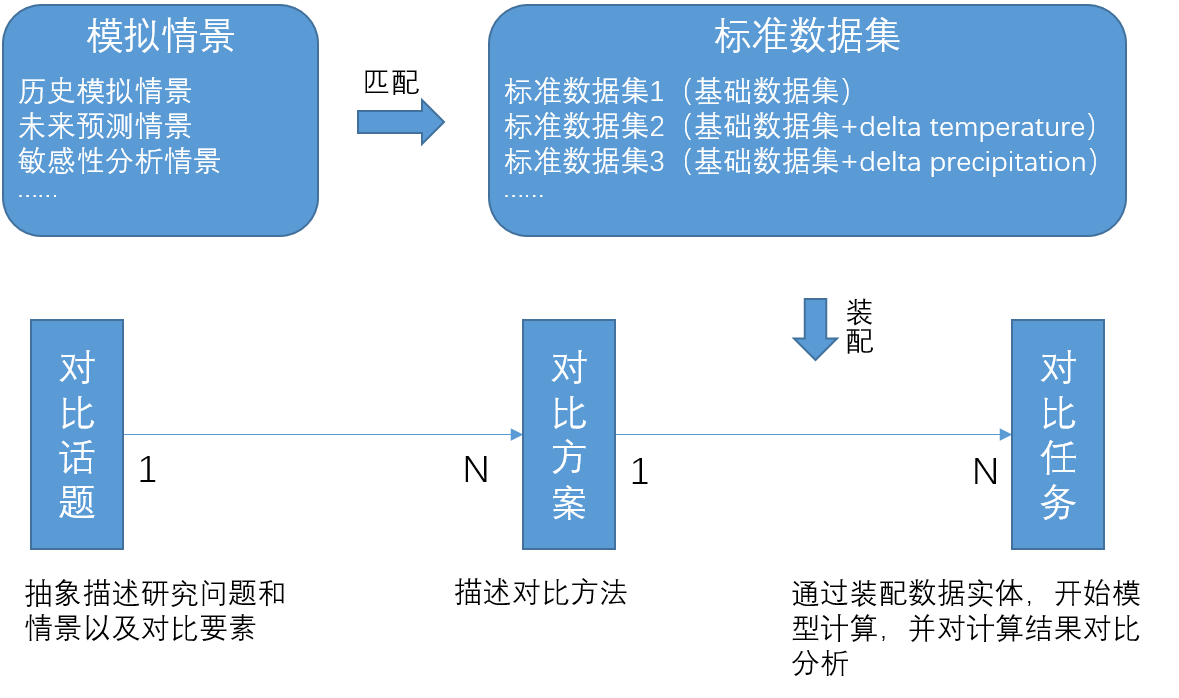
\includegraphics[width=1\textwidth]{cmip-business-abstraction}
    \caption{陆地生态系统碳循环模型对比业务抽象和归纳}
    \label{fig:cmip-business-abstraction}
\end{figure}

陆地生态系统碳循环模型在各种情景中可以归纳出三个主要关注点:研究问题、对比方法和模型运行数据的设定。这三点可以抽象为对比话题、对比方案和对比任务三个层次,如图~\ref{fig:cmip-business-abstraction}所示,对比业务的开展对应为对比话题、对比方案和对比任务创建和执行上。其中,\textbf{对比话题}中指明了研究问题、对比情景和对比要素;\textbf{对比方案}配置了对比参与者和对比方法,对比方案不包括具体的输入数据、观测数据和模拟结果,他表示的仅仅是对比的配置项,从而实现对比过程的可共享性、可重用性和可重现性;\textbf{对比任务}描述的是对比方案配置输入数据和观测数据实体的结果。模型在对比任务中开始具体的运算,并将运算结果与观测数据进行统计学对比和可视化对比。1个对比话题可以对应多个对比方案,一个对比方案通过配置不同的标准数据集可以对应多个对比任务。图~\ref{fig:UML-topic-solution-task}展示了对比话题、对比方案和对比任务的详细接口设计。

\begin{figure}[!htbp]
    \centering
    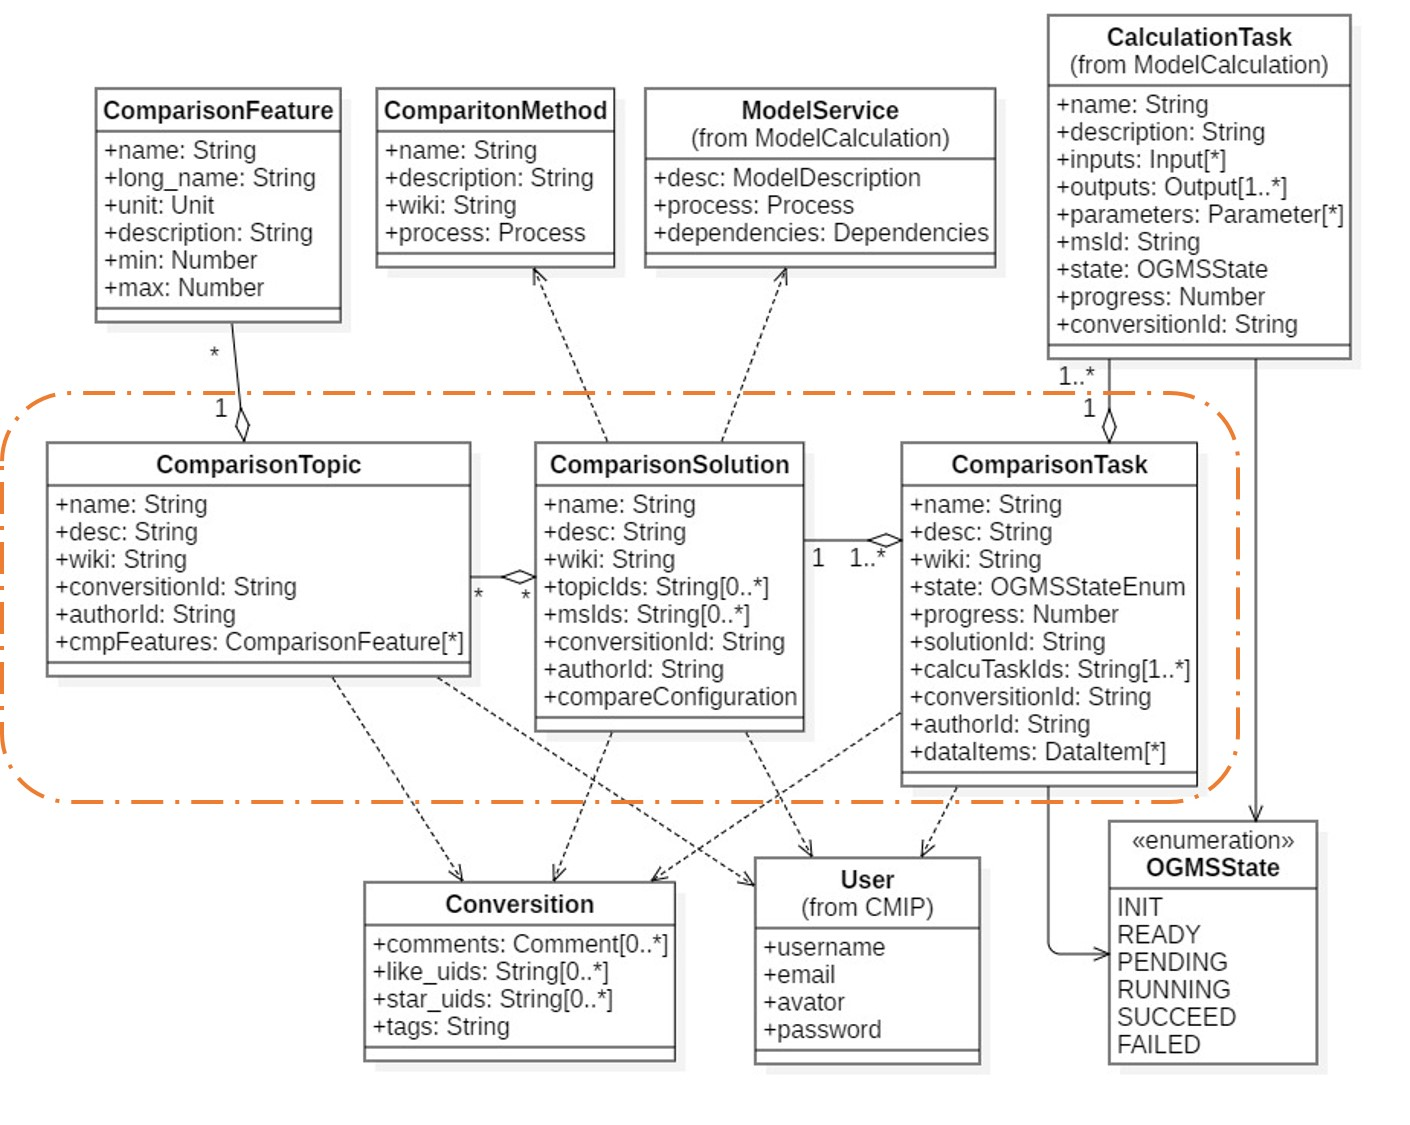
\includegraphics[width=1\textwidth]{UML-topic-solution-task}
    \caption{对比话题、对比方案和对比任务的接口设计UML图}
    \label{fig:UML-topic-solution-task}
\end{figure}

以植被生产力的对比为例,如表\ref{tab:topic-solution-task-example}所示,针对全球历史时期的植被生产力创建一个对比话题,对比要素包括有GPP、NPP、NEP等,这一个话题关联两个对比方案,其中对比参与者相同,都是IBIS、Biome-BGC和LPJ三个模型,第一个方案研究的是站点尺度,它使用的对比方法包括统计学和可视化两大类,通过配置不同的站点数据可以对应231个对比任务;第二个方案研究的是全球范围,它使用的对比方法只有可视化对比方法,只能创建一个相应的对比任务。这样的三层抽象使对比方案可共享与重用,简化了模型对比的难度,并将最后的对比结果公开发布为服务,使对比过程公开透明,更加具有可信度。

% TODO 从 pdf 导入吧
\begin{table}
    \centering
    \caption{针对全球植被生产力评估的对比话题、对比方案和对比任务}
    \label{tab:topic-solution-task-example}
    \begin{threeparttable}
        \begin{tabular}{l | l | l | l | l }
            \Xhline{1.5pt}
            \multicolumn{2}{c}{\makecell[b]{对比话题}} & \multicolumn{2}{|c|}{\makecell[b]{对比方案}} & \multicolumn{1}{l}{\makecell[b]{对比任务}} \\
            \hline
            模拟情景 & 对比要素 & \makecell{对比参与者} & \makecell{对比方法} & 数据区域 \\
            
            \Xhline{1.5pt}
            \multirow{3}{*}{历史情景} & \multirow{3}{2cm}{GPP \quad NPP \quad NEP\ } & \multirow{3}{*}{\makecell{IBIS\\Biome-BGC\\LPJ}} & \multirow{2}{*}{\makecell{统计学对比方法\\可视化对比方法}} & CN-Cha(长白山)站点 \\
            \cline{5-5}
            &  &  &  & 其他站点,共231个 \\
            \cline{4-5}
            &  &  & 可视化对比方法 & 全球 \\
            \Xhline{1.5pt}
        \end{tabular}
    \end{threeparttable}
\end{table}

\subsection{对比系统功能模块设计}
本文将系统的主要功能模块设计为如图\ref{fig:system-module},功能模块分为资源模块、对比业务模块、结果展示模块和用户模块,其中资源模块包括模型资源和数据资源,对比业务模块则对应于对比话题、对比方案和对比任务,结果展示模块基于所有对比任务的对比结果,以网站的形式发布出去。

\begin{figure}[!htbp]
    \centering
    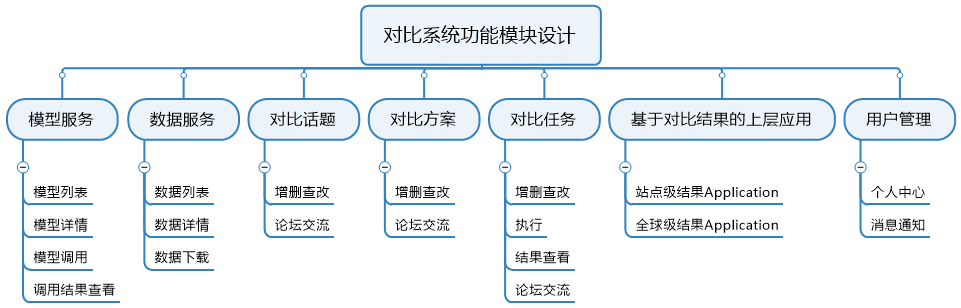
\includegraphics[width=1\textwidth]{system-module}
    \caption{对比系统功能模块设计}
    \label{fig:system-module}
\end{figure}

\section{基于服务的开放式地理资源库}
% GIS的发展:硬耦合->组件->服务
% 本文的架构:服务式、服务化的意义
% REST API

% 自60年代Tomlinson首先提出GIS并建立世界上第一个地理信息系统开始,GIS已经取得了突飞猛进的发展,从最开始的面向土地信息管理的GIS到适用于各种各样丰富专题如城市规划、交通管理、自然资源管理等的GIS。GIS在系统构建经历了从集成式到组件式再到基于服务的Web GIS的发展历程。其中集成式GIS功能丰富全面但系统复杂、庞大、成本高昂,而且不能与其他系统集成;组件式GIS通过多元空间数据无缝集成技术(Seamless Integration of Multisource Spatial-data,SIMS)解决了多源异构数据的访问,并且具有可扩展、可共享和可重用能力,但是组件只能应用于本地计算机;基于Web Service的Web GIS则通过定义空间数据和模型的标准描述协议,实现了数据、模型及计算资源的共享,具备可扩展性、跨平台性,使GIS真正实现大众化。本文的对比系统基于Web Service技术,通过服务实现陆地生态系统碳循环模型的在线对比,一方面实现了地理资源的开放式共享和重用,另一方面也可以使对比过程公开化、透明化,使对比结果能够方便地复现。下面将详细介绍本文中的开放式地理资源库。

\subsection{模型服务资源库}
% 这里介绍所有API,第四章详细介绍模型服务的调用API
地理模型服务资源库包括有一系列陆地生态系统碳循环模型发布出的服务,

\begin{table}
    \centering
    \caption{模型服务API}
    \label{tab:model-service-API}
    \begin{threeparttable}
        \begin{tabu} to 1\hsize{X}
            \Xhline{1.5pt}
            \Xhline{1.5pt}
            \Xhline{1.5pt}
        \end{tabu}
    \end{threeparttable}
\end{table}

\subsection{数据服务资源库}

数据服务资源库包括第标准输入数据集、衍生输入数据集和结果数据集。

\begin{table}
    \centering
    \caption{数据服务API}
    \label{tab:model-service-API}
    \begin{threeparttable}
        \begin{tabu} to 1\hsize{X}
            \Xhline{1.5pt}
            \Xhline{1.5pt}
            \Xhline{1.5pt}
        \end{tabu}
    \end{threeparttable}
\end{table}

\subsection{单位量纲资源库}


% \renewcommand{\arraystretch}{1.5}
% TODO min and max
\begin{table}[!htbp]
    \caption{对比要素及其单位量纲}
    \label{tab:std-metrics}
    \begin{subtable}[t]{.6\linewidth}
        \centering
        \caption{陆地生态系统碳水循环要素表}
        \label{tab:c-w-feature}
        \begin{tabular}{llrrr}
            \Xhline{1.5pt}
            \textbf{名称} & \textbf{单位} & \textbf{最小值} & \textbf{最大值}  \\
            \Xhline{1.5pt}
            $GPP$ & $gC m^2 d^{-1}$ & 0 & 100 \\
            $NPP$ & $gC m^2 d^{-1}$ & 0 & 100 \\
            $NEP$ & $gC m^2 d^{-1}$ & -100 & 100 \\
            $NEE$ & $gC m^2 d^{-1}$ & -100 & 100 \\
            $Biomass$ & $gC m^2 d^{-1}$ & 0 & - \\
            $R_A$ & $gC m^2 d^{-1}$ & 0 & 100 \\
            $R_H$ & $gC m^2 d^{-1}$ & 0 & 100 \\
            $ET$ & $mm d^{-1}$ & 0 & 100\\
            $Runoff$ & $mm d^{-1}$ & - & - \\
            $LAI$ & $1$ &  & \\
            \Xhline{1.5pt}
        \end{tabular}
    \end{subtable}%
    \begin{subtable}[t]{.3\linewidth}
        \centering
        \caption{单位量纲表}
        \label{tab:unit-dimension}
        \begin{tabular}{ll}
            \Xhline{1.5pt}
            \textbf{单位} & \textbf{量纲}  \\
            \Xhline{1.5pt}
            \multirow{3}{*}{$gC m^2 d^{-1}$} & 质量($M$) \\
            & 长度($L$) \\
            & 时间($T$) \\
            \hline
            \multirow{2}{*}{$mm d^{-1}$} & 长度($L$) \\
            & 时间($T$) \\
            \Xhline{1.5pt}
        \end{tabular}
    \end{subtable}
\end{table}

\subsection{数据重构服务资源库}



\subsection{可视化服务资源库}



\subsection{对比服务资源库}


\section{基于微服务的分布式网络架构设计}
% 开放性应体现在:可共享和重用(业务流程归纳)、计算和对比过程公开化(服务化)、模型和数据资源可扩展(微服务注册和发现)、大规模计算场景下体系稳定可用(微服务LB)、自动化易用(科学工作流)
分布式将不同物理区域的计算资源组织整合起来,与传统的集中式相对比,分布式能够有效利用多个分布式节点上的计算能力和数据共享能力,从而提高服务端的性能。
微服务是一种分布式的系统架构风格,由Martin Fowler提出~\cite{fowler2014microservices},微服务是颗粒比较小的服务,一个大型的复杂软件可以由多个微服务组成。微服务采用UNIX的设计哲学,每种服务只做一件事,是一种松耦合的能够被独立开发和部署的无状态化服务。微服务通过服务来实现应用的组件化,微服务中将组件定义为可被独立替换和升级的软件单元,在应用架构设计中通过将整体应用切分成可独立部署的微服务方式进行组件化设计。这种设计方式使得应用程序效率高、灵活性强、可用性高、可扩展性强。

本文基于微服务的分布式网络架构,设计了三种服务器:计算服务器、对比服务器和资源服务器,如图\ref{fig:network-archecture}所示,计算服务器负责模型服务的发布、注册、管理和调用;对比服务器作为门户网站的后台服务器,负责资源的汇总与展示、对比话题和方案的创建、计算任务的分发和对比结果的展示;资源服务器负责数据相关操作,包括数据存储、数据库管理、数据服务的发布和结果数据的缓存。其中计算服务器对外提供模型微服务,资源服务器对外提供数据微服务,三者通过资源交换和消息通信完成协同完成对比任务。

\begin{figure}[!htbp]
    \centering
    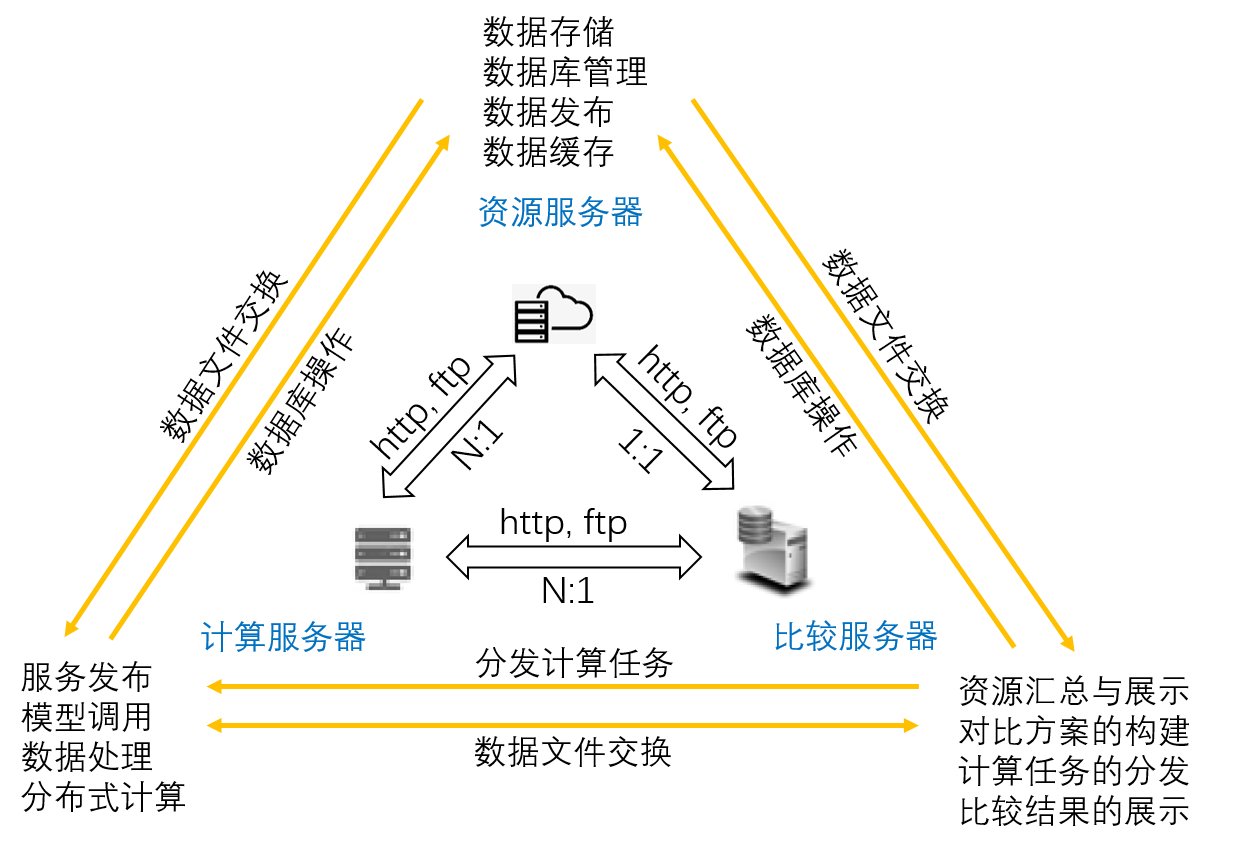
\includegraphics[width=1\textwidth]{network-archecture}
    \caption{分布式网络架构}
    \label{fig:network-archecture}
\end{figure}

\subsection{资源服务器层}
% 功能、特点、服务
资源服务器主要有以下三点功能:
\begin{enumerate}[(1)]
\item \textbf{数据文件存储和缓存}

数据文件包括各种输入数据、对比参照数据和输出数据。模型在运行时从资源服务器请求输入数据,运行结束后将输出数据存储到资源服务器。对比任务执行时从资源服务器请求模型输出数据和对比参考数据,并将对比结果的图表存储到资源服务器。

\item \textbf{数据库存储管理}

整个对比系统的数据库存放在资源服务器上,数据库选择的是MongoDB,通过MongoDB Wire Protocol协议对计算服务器和对比服务器上的客户端开放。

\item \textbf{数据服务的发布}

资源服务器使用OGC WMS/WFS/WCS对外发布地图服务、矢量和栅格数据服务,从而实现空间数据的查询、预览。

\end{enumerate}

资源服务器作为微服务的服务提供者,将这些功能通过微服务的方式对外发布,如图~\ref{fig:resource-server-microservice}所示,计算服务器、对比服务器以及客户端浏览器以对应的协议请求微服务。针对这些功能,资源服务器的硬件配置要求是硬盘大,网络带宽高,以方便数据存储和交换。

\begin{figure}[!htbp]
    \centering
    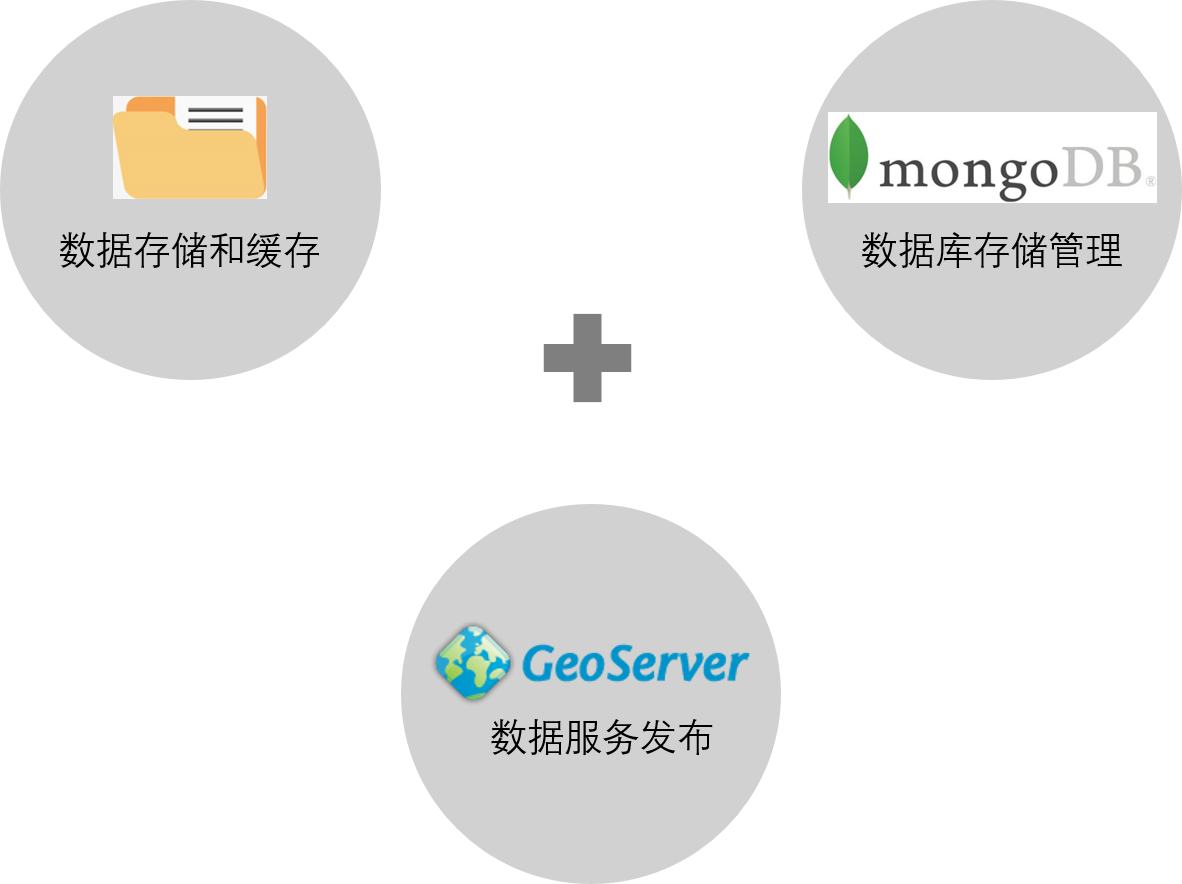
\includegraphics[width=1\textwidth]{resource-server}
    \caption{资源服务器功能}
    \label{fig:resource-server}
\end{figure}

\begin{figure}[!htbp]
    \centering
    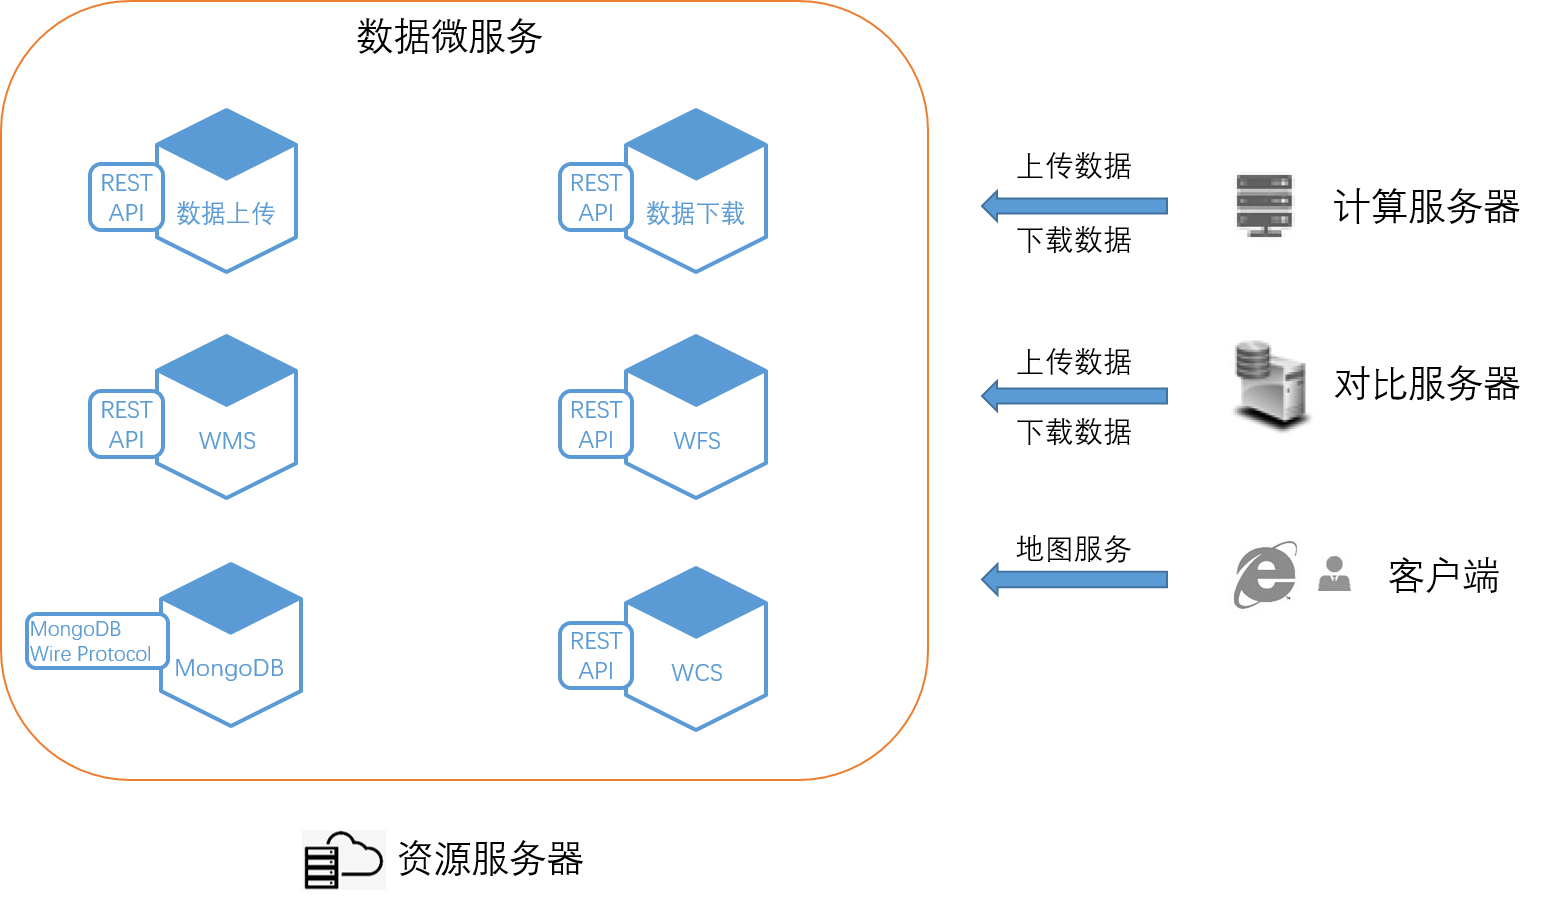
\includegraphics[width=1\textwidth]{resource-server-microservice}
    \caption{资源服务器微服务}
    \label{fig:resource-server-microservice}
\end{figure}


\subsection{计算服务器层}
计算服务器的主要功能是模型服务的发布、注册、管理和调用,针对这些功能,需要在服务器上部署计算服务容器,如图~\ref{fig:ms-server-microservice}所示,计算服务容器由Node.js和MongoDB开发。Node.js对外暴露模型调用的接口,当客户端经过HTTP协议发送调用请求时,在计算服务容器内部调用模型应用程序。当模型运行结束后,计算服务容器获取子程序的句柄,将运行结果的状态保存到MongoDB中。模型微服务与数据微服务有一些不同之处:每个独立的模型服务可以根据软硬件需求存放在不同的服务器上,即模型微服务有多计算节点的特性。因此,模型微服务发布后,还需要将服务注册到模型服务资源库中,从而能够被服务消费者发现服务。

\begin{figure}[!htbp]
    \centering
    \subcaptionbox{模型微服务的发布和调用}{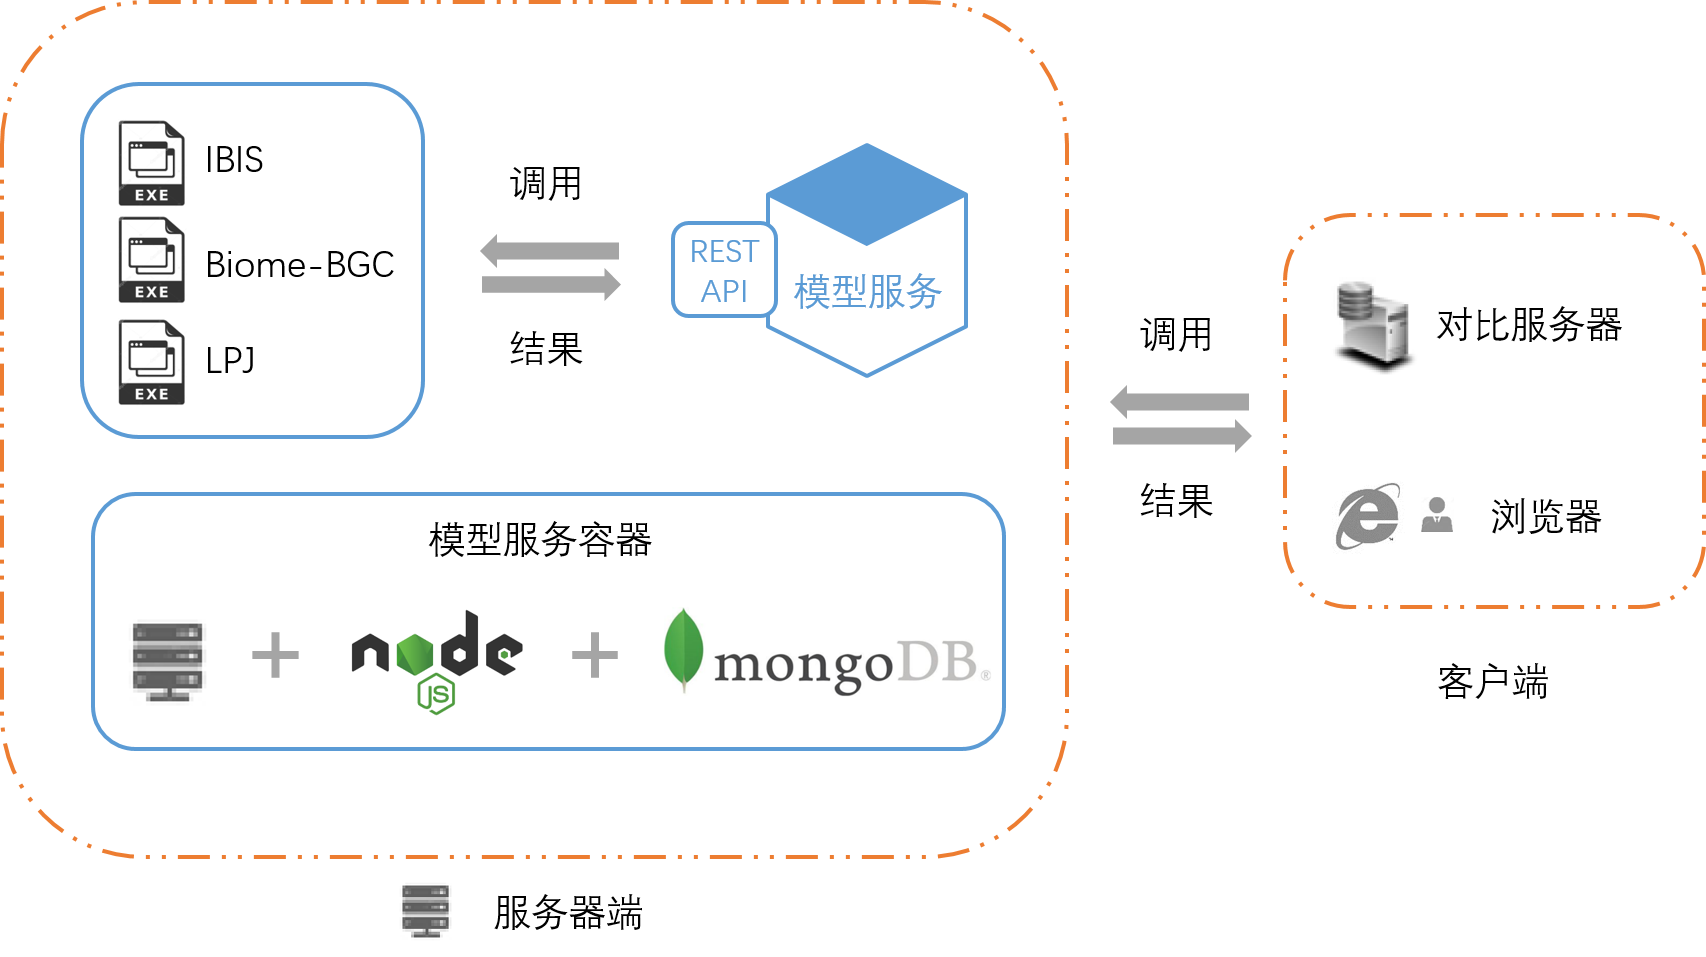
\includegraphics[width=0.65\textwidth]{ms-server-microservice-a}}
    \hfill
    \subcaptionbox{模型微服务多节点分布}{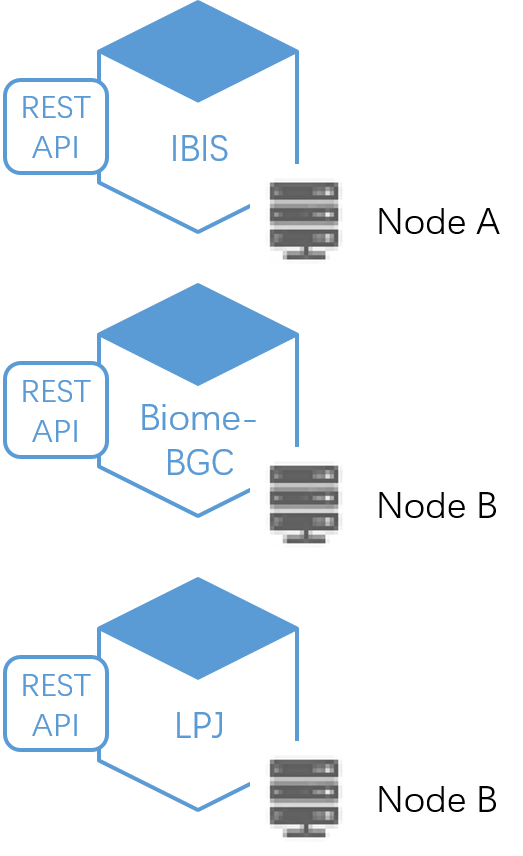
\includegraphics[width=0.25\textwidth]{ms-server-microservice-multi-nodes}}
    \caption{计算服务器微服务}
    \label{fig:ms-server-microservice}
\end{figure}

\subsection{对比服务器层}
对比服务器的主要功能是分发计算任务,并把模型计算出来的结果文件和对比参考数据进行对比。他是模型微服务和数据微服务的消费者、对比微服务的生产者。如图~\ref{compare-server-microservice}所示,模型对比的开展主要包括以下几步:

\begin{enumerate}[(1)]
\item 用户在浏览器客户端通过HTTP协议发送对比任务的调用请求;
\item Node.js的路由器收到请求后,将对比任务中包含的计算任务拆分出来,并通过调用计算服务器上的模型微服务启动计算任务,并不断轮询监控模型的运行进度;
\item 当监测到所有模型都运行成功后,从资源服务器上发布的模型运行结果微服务和对比参考数据微服务下载数据,然后调用本地的对比方法脚本程序,这些脚本可由JavaScript、Python或Matlab等编写而成;
\item 最后将对比脚本的结果文件保存到数据库中,并返回给客户端。
\end{enumerate}

另外他作为门户网站的后台服务器,还负责浏览器前台的一系列操作,如资源汇总与展示、对比流程的创建、对比结果的展示等。

\begin{figure}[!htbp]
    \centering
    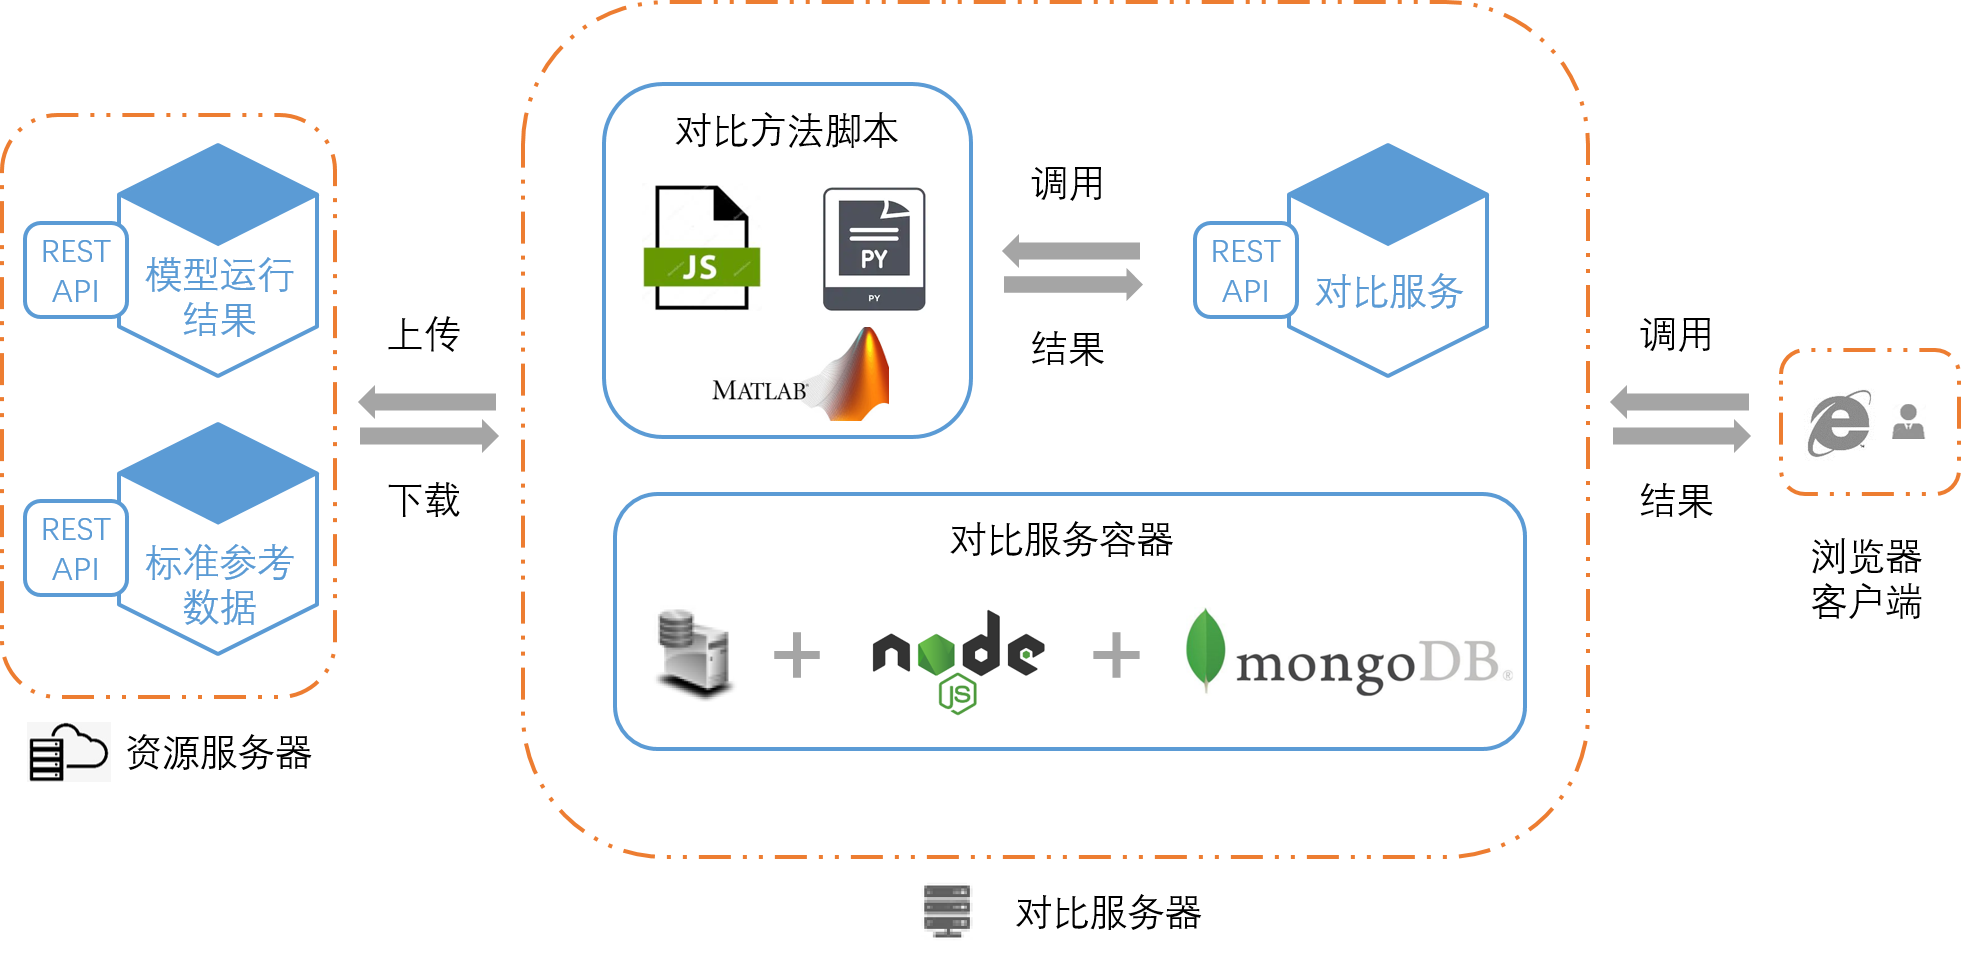
\includegraphics[width=1\textwidth]{compare-server-microservice}
    \caption{对比服务器微服务}
    \label{fig:compare-server-microservice}
\end{figure}

\subsection{服务器通信}
% 计算节点注册、服务注册、服务发现、服务通信

\section{开放式对比科学工作流引擎}
% % 模型调用-数据缓存-数据重构-数据对比
\subsection{对比流程分析和归纳}
如图~\ref{fig:workflow-example}所示,

\begin{figure}[!htbp]
    \centering
    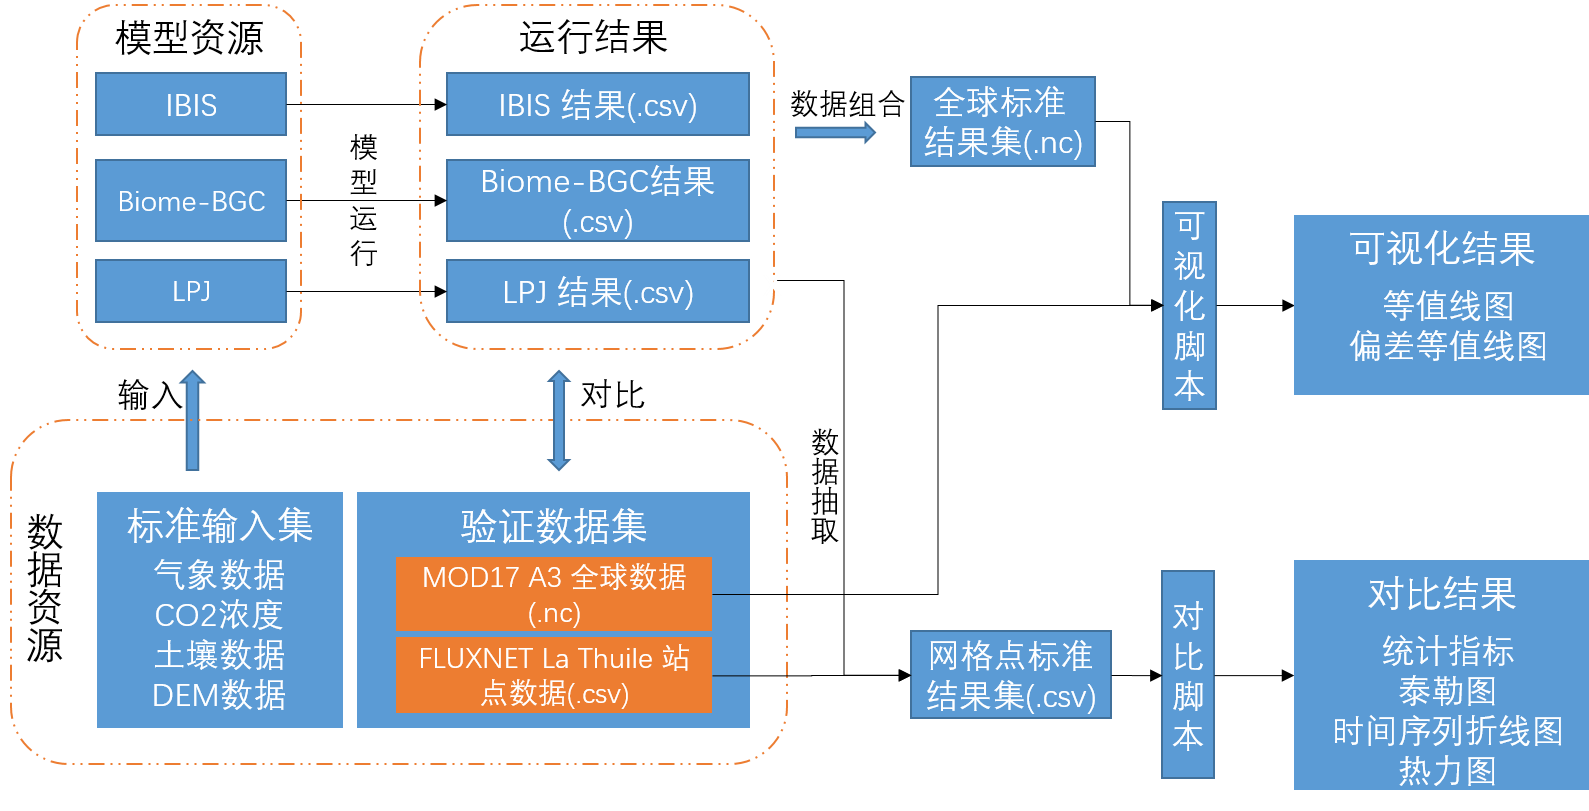
\includegraphics[width=1\textwidth]{workflow-example}
    \caption{以IBIS、Biome-BGC、LPJ三个模型为例的对比流程}
    \label{fig:workflow-example}
\end{figure}

\subsection{对比自动化执行引擎}
% 科学工作流定义、特点
% 本文的应用
工作流是一类能够完全或者部分自动执行的经营过程,根据一系列过程规则,文档、信息、或任务能够在不同的执行者之间传递、执行。科学工作流是工作流的一种,它主要面向科学实验过程,以数据驱动,用来描述和控制科学实验和过程的执行~\cite{ludascher2006scientific}~\cite{Zhao2009Special}。科学工作流的特点是面向数据、数据规模大、具有动态适应性以支持工作流执行过程中的动态资源绑定。本文的对比工作流执行流程如图~\ref{fig:workflow}所示,其中数据服务库中的数据量巨大、存储节点分散,模型服务库中的模型可以动态添加和删除,并通过标准化的接口暴露出来。工作流首先调用模型服务,然后将模型运行出的结果和观测数据交给数据重构服务进行数据重构,将两者的单位量纲统一,并抽取出需要的那一部分,最后通过对比服务对数据进行统计学对比,使用可视化服务对数据进行统计图表和地图形式的展示。

\begin{figure}[!htbp]
    \centering
    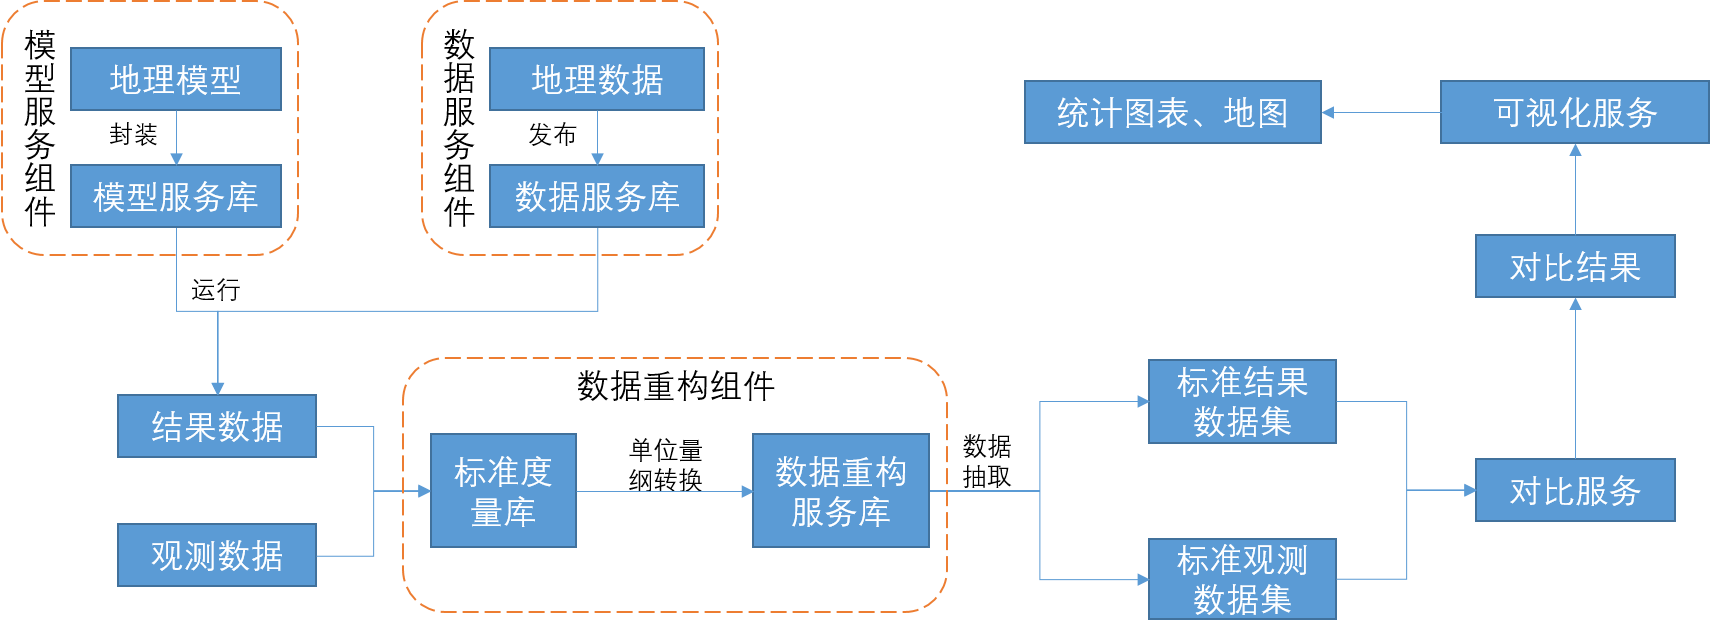
\includegraphics[width=1\textwidth]{workflow}
    \caption{开放式对比科学工作流流程图}
    \label{fig:workflow}
\end{figure}

从微服务的视角来看,如图~\ref{fig:microservice-cmp-integration}所示,对比科学工作流的各个数据处理过程都是一个微服务,并分散在分布式的网络节点上,对比工作流在执行时不用关心数据处理程序的具体网络节点位置,通过微服务暴露的IP地址和端口来寻找计算节点,这样就将分布式节点有效管理起来。

\begin{figure}[!htbp]
    \centering
    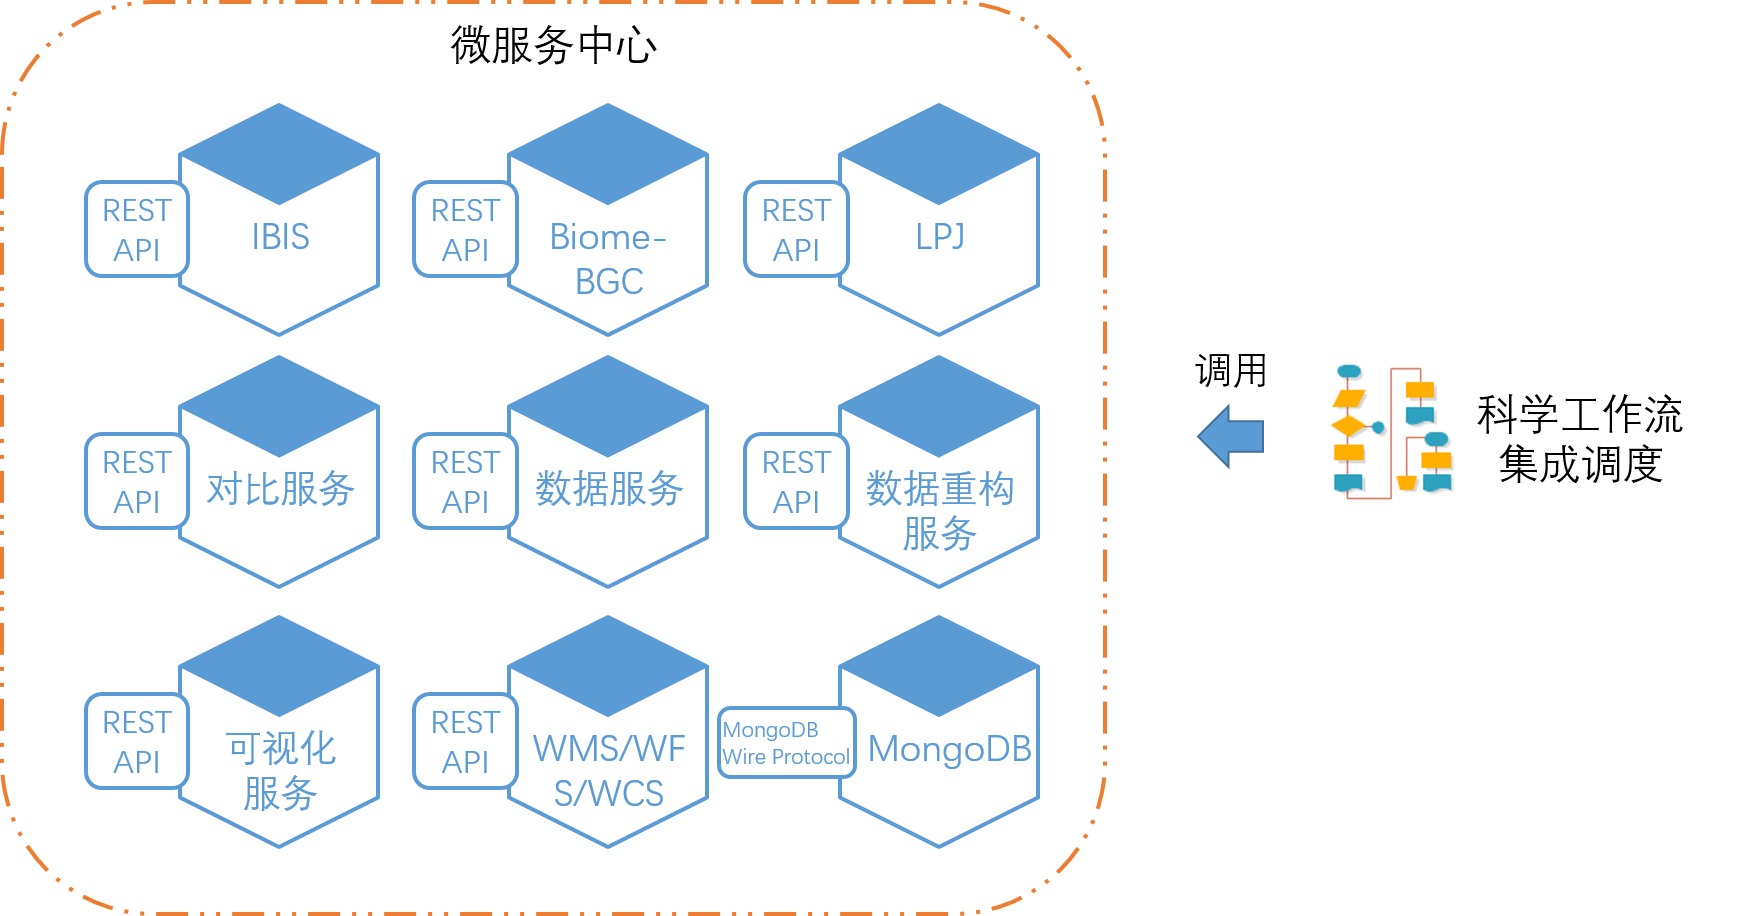
\includegraphics[width=1\textwidth]{microservice-cmp-integration}
    \caption{对比科学工作流引擎和微服务}
    \label{fig:microservice-cmp-integration}
\end{figure}


\section{本章小结}
开放式对比系统的构建有两个关键问题:一是如何设计一个开放式的对比框架,二是这些对比资源如何接入框架。对于问题一,本章从对比业务、资源组件、网络架构和执行引擎四个角度进行了详细论述,设计的系统框架具有以下特点的:

\begin{enumerate}[(a)]
    \item 模型计算和对比可共享与重用;
    \item 模型计算和对比过程公开化;
    \item 模型和数据资源可扩展性地动态接入;
    \item 大规模计算场景下稳定可用;
    \item 以自动化实现其易用性。
\end{enumerate} 

对于问题二将在下一章详细论述。